\documentclass{article}

%%%%%%%%%%%%%%% LIBRERIAS %%%%%%%%%%%%%%%%%%%%%
\usepackage{amsmath}
\usepackage{titlesec}
\usepackage{titletoc}
\usepackage{graphicx}
\usepackage[spanish,es-tabla]{babel} % 'es-tabla' cambia Cuadro→Tabla
\usepackage{hyperref}                % cargar después de babel
\usepackage{float}
\usepackage{circuitikz}
\usepackage[left=3cm,right=3cm]{geometry} %para margenes
%%%%%%%%%%%%%%%%%%% VARIABLES %%%%%%%%%%%%%%%%%%%%
\newcommand{\Facultad}{Instituto Tecnológico \\de\\ Buenos Aires} %constantes
\newcommand{\TPn}{Trabajo Práctico N° 3}
\newcommand{\TPtema}{Respuesta Transitoria}
\renewcommand{\thesection}{\arabic{section}}          % 2
\renewcommand{\thesubsection}{\quad \alph{subsection}}   % a
\renewcommand{\thesubsubsection}{\quad \thesubsection.~\roman{subsubsection}} % a. i
\graphicspath{{imagenes/}} %para que acceda a las fotos en la carpeta directamente


%%%%%%%%%%%%%%%%%% FORMATO TÍTULO Y NUMERACIÓN %%%%%%%%%%%%%%%%%%%
% Numeración de secciones
\renewcommand{\thesection}{\arabic{section}.}          
\renewcommand{\thesubsection}{\thesection\arabic{subsection}}       
\renewcommand{\thesubsubsection}{$\alph{subsubsection})$}

% Numerar hasta subsubsecciones
\setcounter{secnumdepth}{3}

% Formato de títulos
\titleformat{\section}{\Huge\bfseries}{\thesection}{1em}{}
\titleformat{\subsection}{\LARGE\bfseries}{\thesubsection}{0.5em}{}
\titleformat{\subsubsection}{\large\bfseries}{\thesubsubsection}{0.5em}{}



%%%%%%%%%%%%%%%%%%% ARCHIVO %%%%%%%%%%%%%%%%%%%%%%%%
\begin{document}

%%%CARATULA%%%
\begin{titlepage} %creo portada

        \begin{flushleft}
            \centering
            
\includegraphics[width=0.3\textwidth]{Logo_ITBA.png}
        \end{flushleft}

        \centering
            
        {\scshape\LARGE \Facultad \par} %\par sirve para indicar un final de parrafo
        \vspace{1cm}                    %esto hace un espacio entre lineas de 1cm


        {\huge\bfseries \TPn \par}
        \vspace{1.5cm}
        {\Large Teoría de Circuitos I\\ 25.10 \par}
        \vfill                      %sirve para rellenar el espacio y quede simétrico. Si se añaden otros, se dividen el espacio de forma equitativa
        {\Large \bfseries Grupo N° 2 \par}
        \vspace{1cm}
        {\large Juan Bautista Correa Uranga \hfill Legajo: 65016 \par} %\hfill sirve para hacerlo simétrico
        {\large Juan Ignacio Caorsi \hfill Legajo: 65532  \par}
        {\large Rita Moschini \hfill Legajo: 67026 \par} 
        \vfill
        {\large \today\par}
        \vfil

    \end{titlepage}

 %%%RESUMEN%%%
{\centering \LARGE \bfseries Resumen \par}

\newpage

%%%INDICE%%%
\tableofcontents %esto sirve para crear el índice

\newpage

%%%Introduccion%%%
\section{Introducción}
    Este trabajo práctico aborda la respuesta transitoria
     en circuitos RLC serie. Se busca aplicar conceptos 
     teóricos mediante mediciones reales, utilizando generador 
     de señales y osciloscopio. Se analiza cómo varían las
      respuestas al modificar resistencia, inductancia y 
      capacitancia, observando casos de subamortiguamiento,
       sobreamortiguamiento y amortiguamiento crítico. 
       El objetivo es comprender la dinámica temporal 
       de circuitos RLC y validar modelos teóricos
       con datos experimentales.
    \subsection{Instrumental}
        En esta experiencia se utilizaron los siguientes instrumentos:
\begin{itemize}
  \item Osciloscopio Keysight DSOX 1202G con generador de ondas integrado.
  \item Capacitores de $47\,\text{pF}$ y $470\,\text{pF}$.
  \item Resistencias de 220 $\Omega$ nominal y potenciómetro de 5 k$\Omega$ nominal.
  \item Inductor de resistencia indefinida, con inductancia aproximada de $1\,\text{mH}$.
  \item Multímetro UNI-T,  Standar Digital multimeter, modelo: UT39C.
\end{itemize}

    \subsection{Marco teórico}

        Un circuito RLC serie está compuesto por una resistencia (R),
         una 
        inductancia (L) y una capacitancia (C) conectadas en serie.
        Dependiendo de la resistencia del circuito, la respuesta transitoria
         puede ser subamortiguada, sobreamortiguada o críticamente 
         amortiguada. La ecuación diferencial que describe la 
         respuesta del circuito RLC serie es:
        \begin{equation}
            L\frac{d^2i(t)}{dt^2} + R\frac{di(t)}{dt} + \frac{1}{C}i(t) = V_{in}(t)
        \end{equation}

        y su solución general es la suma de la respuesta natural y la respuesta forzada:

Para la respuesta natural (\( V_{\text{in}}(t) = 0 \)), se define:

\begin{equation}
\alpha = \frac{R}{2L}, \quad \omega_0 = \frac{1}{\sqrt{LC}}, \quad \Delta = \alpha^2 - \omega_0^2
\end{equation}

La solución general depende del valor de \( \Delta \):

\begin{itemize}
  \item \textbf{Sobreamortiguado} (\( \Delta > 0 \)):

  \begin{equation}
  i(t) = A e^{(-\alpha + \sqrt{\Delta})t} + B e^{(-\alpha - \sqrt{\Delta})t}
  \end{equation}

  \item \textbf{Críticamente amortiguado} (\( \Delta = 0 \)):

  \begin{equation}
  i(t) = (A + Bt)e^{-\alpha t}
  \end{equation}

  \item \textbf{Subamortiguado} (\( \Delta < 0 \)):

  \begin{equation}
  i(t) = e^{-\alpha t} \left( A \cos(\omega_d t) + B \sin(\omega_d t) \right)
  \end{equation}

  donde \( \omega_d = \sqrt{\omega_0^2 - \alpha^2} \).
\end{itemize}

%%%Desarrollo%%%
\section{Desarrollo}
    \subsection{Procedimiento}

\begin{figure}[H]
    \centering
    \begin{tikzpicture}
        \draw (15.75, -14.5) to[american voltage source, l={$Vs$}] (15.75, -17.75);
        \draw (15.75, -14.5) to[american resistor, l={$Rf$}] (19.5, -14.5);
        \draw (19.5, -14.5) to[variable american resistor, l={$Rv$}] (22.25, -14.5);
        \draw (22.25, -14.5) to[cute inductor, l={$L$}] (22.25, -17.75);
        \draw (22.25, -17.75) to[capacitor, l={$C$}] (15.75, -17.75);
    \end{tikzpicture}
    \caption{Circuito analizado}
    \label{fig: circuito_rlc}
\end{figure}


    La parte experimental se realizó en una serie de 4 pasos:

    \begin{enumerate}
        \item Primero se armó el circuito en serie (observar figura \ref{fig: circuito_rlc}) usando el capacitor de 470 pF. Luego de esto, se procedió con su análisis variando el valor de la resistencia variable. Finalmente, se determinó de manera aproximada el valor de la resistencia variable que producía un amortiguamiento crítico.
        \item En esta parte, se ajustó la resistencia Rv a su valor máximo. Posteriormente, se calculó de forma experimental el valor $\tau$ del sistema. Con este valor aproximado, se midió la salida en el tiempo $ 5\tau$.
        \item A continuación, se remplazo el capacitor por uno de 47pF. Luego de esto, se observó la respuesta del sistema en función del valor de la resistencia variable. Al mismo tiempo, se repitió la medición del amortiguamiento crítico y se calculó el tiempo del transitorio, pero esta vez, para el valor de Rv mínimo. También se midió la frecuencia y el valor pico.
        \item Finalmente, se cortocircuitaron las resistencias y se analizó la respuesta transitoria nuevamente.
        
    \end{enumerate}
    \subsection{Mediciones}
 
        \begin{itemize}
            \item $ R_f = 215 \Omega $
            \item $ R_{V_{max}} = 9980 \Omega $
            \item $ R_{V_{min}} = 2 \Omega $
            \item $ R_L = 0,8 \Omega $
            \item $ L \approx 1 mH $
        \end{itemize}
        
        \par
        \subsubsection*{Capacitor de C = 470 pF}
            \begin{itemize}
                \item Resistencia variable tal que el amortiguamiento fue crítico: $ R_{critico} = 1,9 k\Omega $ % item 1
                \item Tiempo $\tau$ en que la salida llegó a 3,175 V con $ R_V $ en su valor máximo: $ \tau = 5,75 \mu s$ % item 2
                \item Salida cuando $t=5\tau$ con $ R_V $ en su valor máximo: $V_{5\tau}$ = 5 V% item 2
            \end{itemize}

        \par
        \subsubsection*{Capacitor de C = 47 pF}
            \begin{itemize}
                \item Resistencia variable tal que el amortiguamiento fue crítico: $ R_{critico} = 3,47 k\Omega $ %item 3
                \item Tiempo en que la salida llegó a 3,175 V con $ R_V $ en su valor crítico: $ t = 2,20 \mu s$ % item 3
                \item Tiempo en que la salida llegó a 5,24 V con $ R_V $ en su valor mínimo: $ t = 14,30 \mu s$ % item 4
                \item Tiempo en que la salida llegó a 4,982 V ($ 5V \pm 0,05V $) con las resistencias cortocircuitadas: $ t = 11 \mu s$ % item 5
            \end{itemize}

    \subsection{Cálculos}

        \subsection{Ecuaciones utilizadas}            

            \textbf{Cálculo del la resistencia variable tal que el amortiguamiento fuera crítico} \par \par
            $ \alpha_{serie} = \omega_0 \Rightarrow \frac{R}{2L} = \frac{1}{\sqrt{LC}}  $
            \begin{equation}
                R = \frac{2L}{\sqrt{LC}}
            \end{equation}  \par \par 

            \textbf{Cálculo de la inductancia} \par \par
            Tomando la resistencia variable tal que el amortiguamiento resultase crítico,
            $ R = \frac{2L}{\sqrt{LC}} = 2\frac{\sqrt{L}}{\sqrt{C}} $
            \begin{equation}
                L = \frac{C \cdot R^2}{4}
            \end{equation}

            
        \subsection{Resultados}

            \subsubsection*{Capacitor de C = 470 pF}
                0) Inductancia L
                \begin{equation}
                    L=0.526mH
                \end{equation}
                1) Resistencia variable tal que el amortiguamiento fuera crítico:
                \begin{equation}
                    R_{critico} = 1.857 k\Omega
                \end{equation} \par
                2) $ \tau $ con $ R_V = R_{V_{max}} = 9980 \Omega $:
                 \begin{equation}
                    \tau = 4,74 \mu s 
                \end{equation}

            \subsubsection*{Capacitor de C = 47 pF}
                3) Resistencia variable tal que el amortiguamiento fuera crítico:
                \begin{equation}
                    R_{critico} = 6,47 k\Omega 
                \end{equation} \par
                4) Valor de $ \tau $ para $ R_V = R_{V_{min}} $: 4,83 $\mu$s
                \begin{equation}
                    \tau =  \mu s 
                \end{equation} \par
                6) Valor de $ \tau $ para $ R = R_L $ (resistencias cortocircuitadas): REVISAR
                \begin{equation}
                    \tau =  \mu s 
                \end{equation}
        


    \subsection{Análisis}
    
    	Luego de recolectar los datos, se pudieron observar los siguientes comportamientos. \par
	Es importante mencionar que en este trabajo, no se contó con un valor de referencia de la constante del inductor; esta debió ser aproximada mediante el valor de la resistencia del amortiguamiento critico. Consecuentemente, los datos teóricos también pueden contener errores asociados.
	
        \subsection*{Capacitor 470pF}
        	En esta parte, se observó lo siguiente. Al aproximar el valor de la resistencia del amortiguamiento crítico, se llegó a $1,9k\Omega$, un valor el cual posee un error relativo del 2,32 \% con respecto al valor teórico. Esto indica una buena aproximación al valor real que causa que el sistema sea críticamente amortiguado. \par
	Sumado a esto, se observó que la respuesta se volvía sobreamortiguada al aumentar la resistencia por encima de $1,9k\Omega$ y que la misma se volvía subamortiguada al disminuir la misma por debajo de ese valor. Esto concuerda con las ecuaciones descriptas en el apartado teórico, puesto a que al aumentar R, $\alpha$ aumentaba. \par
	Otras de las áreas analizadas fue la del valor de $\tau$. Esta se aproximó despejando el tiempo el cual llevaba a una respuesta de 3,175 $V$. Se observó que el mismo fue de $5,75\mu F$, un valor el cual posee un error relativo del 21,3\%. Esto muestra un error alto, pero este puede estar asociado en gran medida a la incertidumbre en el valor de la constante L. Al mismo tiempo, dicho $\tau$ teórico se consiguió mediante una aproximación, usando la raíz de la ecuación característica más pequeña y descartando la otra.\par
	Finalmente, se observó que el transitorio en $5\tau$ el valor de la respuesta estaba entre los valores de 4,75 V y 5,25 V. Esto demuestra que la aproximación de $5\tau$ como tiempo de transitorio, es efectiva.
	
	
        \subsection*{Capacitor 47pF}
        En esta parte, se analizó el efecto de la reducción de la capacitancia. Primero se observo que la resistencia del valor crítico aumentaba en comparación con el capacitor de 470pF. Consecuentemente, esto aumentó el margen de valores de las resistencias en los cuales el sistema se mantiene como un subamortiguado.\par
        Al mismo tiempo, también se midió un valor de resistencia que causaba un amortiguamiento crítico. Es valor fue de $3,47k\Omega$, el cual muestra un error relativo del 46,4\%. Este gran error asociado a la medición se debe a que el valor fue obtenido de manera aproximada, sin un ajuste riguroso.\par 
        
        \begin{figure}[h]
    \centering
    \begin{minipage}{0.49\textwidth}
        \centering
        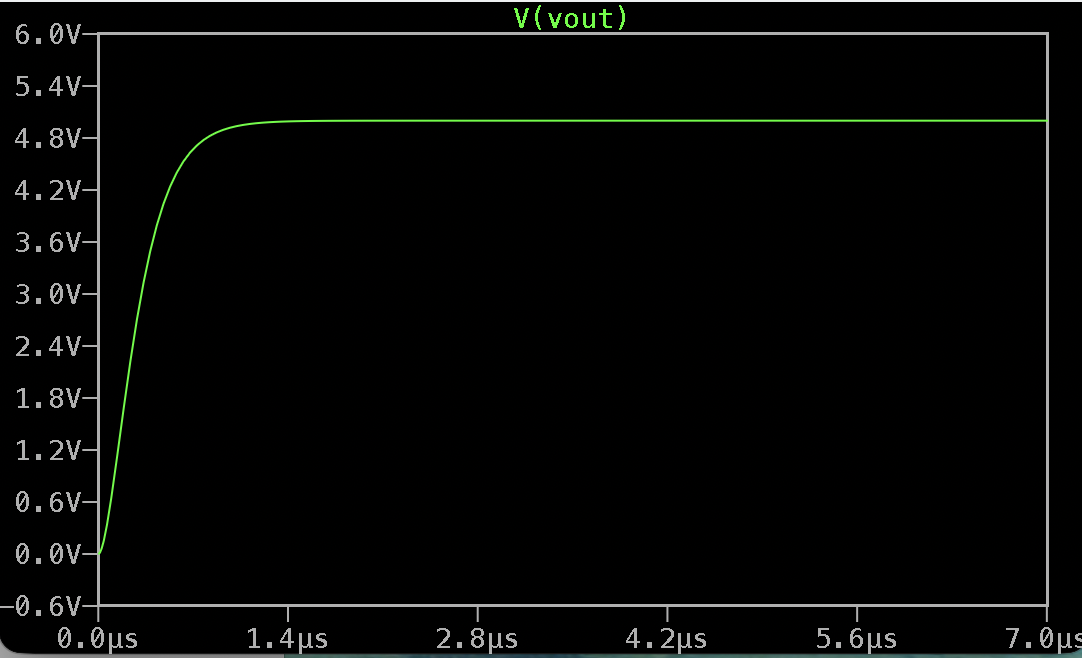
\includegraphics[width=\linewidth]{CRITICAMENTE.png}
        \caption{Capacitor 47pF, con Rv = 6,47 $k\Omega$}
        \label{fig:img1}
    \end{minipage}\hfill
    \begin{minipage}{0.49\textwidth}
        \centering
        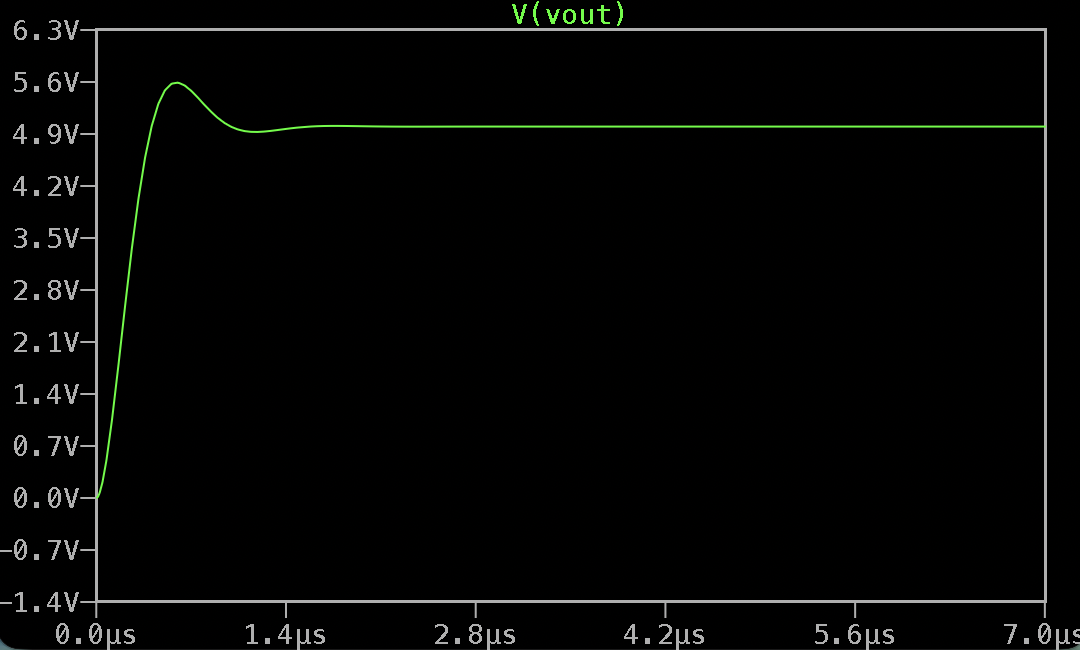
\includegraphics[width=\linewidth]{SUBAMORT.png}
        \caption{Capacitor 47pF, con Rv= 3,47 $k\Omega$}
        \label{fig:img2}
    \end{minipage}
\end{figure}

        Por este motivo, se recurrió a la simulación del mismo usando el valor de L. Es importante volver a mencionar que el mismo ya asocia una gran incertidumbre en su cálculo. Al observar las figuras \ref{fig:img1} y \ref{fig:img2}, se puede observar que el valor calculado mediante el osciloscopio, es un valor subamortiguado. Por tal motivo se considera que el valor de 6,47 $k\Omega$ es el valor aproximado que genera un transitorio críticamente amortiguado.\par
        Por otra parte, al analizar el tiempo de transitorio del sistema, con la resistencia variable configurada en su valor mínimo, se obtuvieron los siguientes datos. El $\tau$ obtenido experimentalmente fue de 14,30 $\mu$s, 
        
        


\section{Conclusiones}

\end{document}